\begin{frame}
\frametitle{Кеширующий аллокатор}
\begin{itemize}
    \item<1->Создадим кеш блоков фиксированного размера
    \begin{itemize}
        \item<2->кеш будет аллоцировать/освобождать большие регионы памяти
        используя другой аллокатор;
        \item<3->кеш "нарезает" большие регионы на блоки фиксированного размера.
    \end{itemize}
\end{itemize}
\end{frame}

\begin{frame}
\frametitle{Кеширующий аллокатор}
\begin{itemize}
    \item<1->Кеширующий аллокатор имеет ряд достоинств:
    \begin{itemize}
        \item<2->фиксированный размер блоков позволяет бороться с фрагментацией;
        \item<3->аллокация/освобождение могут работать за $O\left(1\right)$;
        \item<4->можно скомбинировать кеши разных размеров и построить
        универсальный аллокатор.
    \end{itemize}
\end{itemize}
\end{frame}

\begin{frame}
\frametitle{SLAB}
\begin{itemize}
    \item<1->Кеширующий аллокатор предложенный Джеффом Бонвиком и
    использованный в SunOS (Solaris):
    \begin{itemize}
        \item<2->slab - описывает большой регион памяти, который разбивается на
        маленькие блоки фиксированного размера;
        \item<3->все свободные блоки связываются в список;
        \item<3->количество элементов списка и указатель на первый элемент
        сохраняются в заголовке.
    \end{itemize}
\end{itemize}
\end{frame}

\begin{frame}
\frametitle{SLAB}
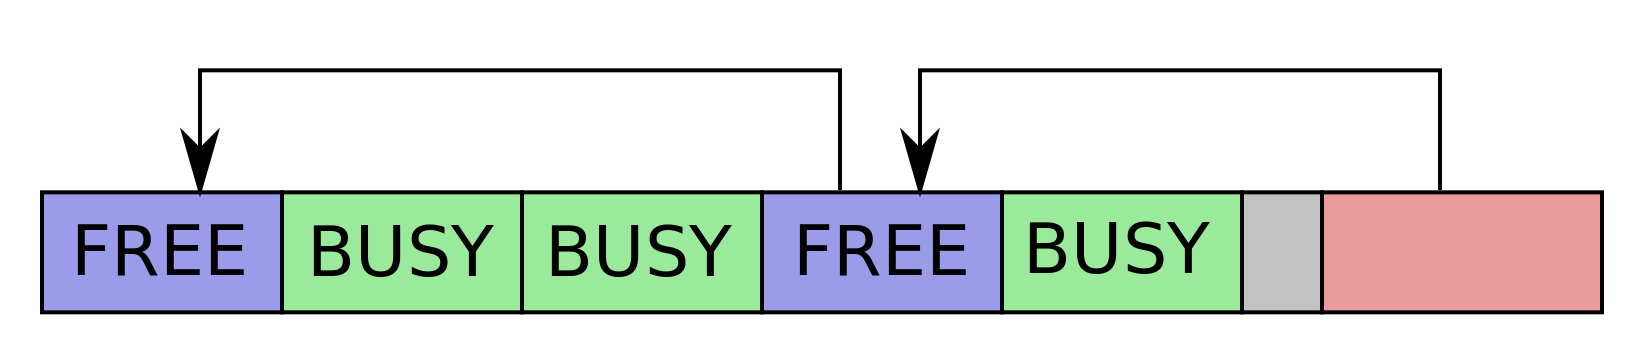
\includegraphics[height=.2\textheight]{slab0}
\end{frame}

\begin{frame}
\frametitle{Управление SLAB-ами}
\begin{itemize}
    \item<1->SLAB аллокатор управляет slab-ами:
    \begin{itemize}
        \item<2->если нет slab-а со свободными объектами - аллоцируем новый;
        \item<3->если все объекты в slab-е свободны - можно освободить slab.
    \end{itemize}
\end{itemize}
\end{frame}

\begin{frame}
\frametitle{Управление SLAB-ами}
\begin{itemize}
    \item<1->SLAB аллокатор поддерживает три списка slab-ов:
    \begin{itemize}
        \item<2->полностью свободные slab-ы;
        \item<3->частично знаятые slab-ы;
        \item<4->полностью занятые slab-ы.
    \end{itemize}
\end{itemize}
\end{frame}

\begin{frame}
\frametitle{Освобождение}
\begin{itemize}
    \item<1->Чтобы освободить элемент нужно найти slab, которому он пренадлежит
    \begin{itemize}
        \item<2->мы можем сохранить указатель на slab рядом с аллоцированной
        памятью;
        \item<3->мы можем потребовать чтобы размер и выравнивание slab-а были
        равны $2^i$.
    \end{itemize}
\end{itemize}
\end{frame}

\begin{frame}
\frametitle{Освобождение}
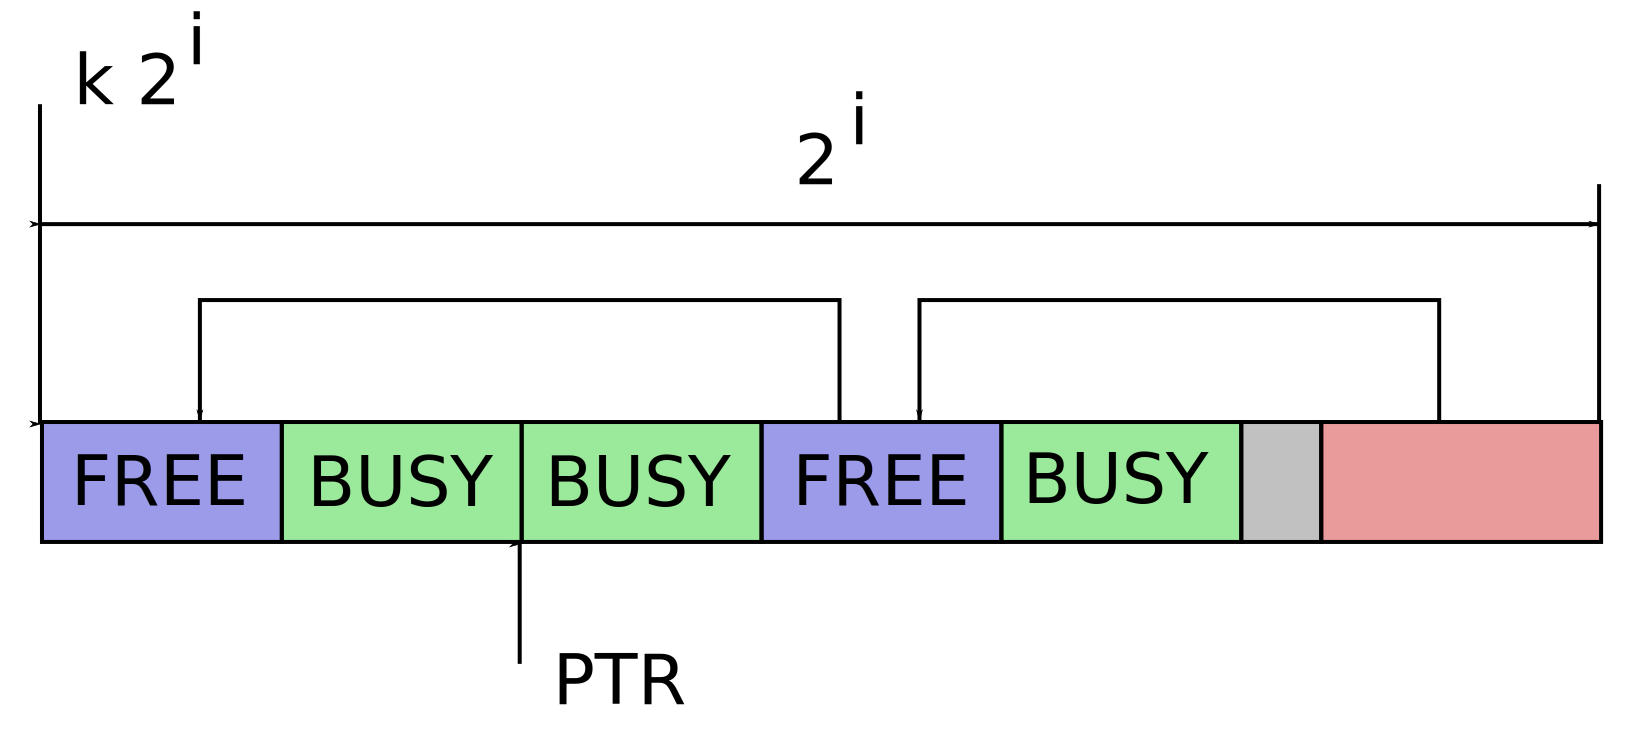
\includegraphics[height=.3\textheight]{slab1}
\end{frame}

